\documentclass[a4paper]{article}

\usepackage[a4paper, total={7in, 10in}]{geometry}
\usepackage[T1,T2A]{fontenc}
\usepackage[utf8]{inputenc}
\usepackage[english,russian]{babel}
\usepackage{mathtools}
\usepackage{graphicx}
\graphicspath{ {./images/} }

\begin{document}

\title{\textit{\textbf{Лабораторная работа №402}}}
\author{Губанов Пётр, С01-019}
\maketitle

\clearpage

\title{\large{\textit{2. Задания к допуску.}}}\\\\

\textbf{\textit{\underline{2.1.}}} Определить максимальную длительность задержки модуля ждущего генератора WGMT в Тсе. \\
$T_{ce}$ меняет своё значение через $MT-1$ промежутков времени длительностью $T_{ce}$ \\

\textbf{\textit{\underline{2.2.}}} Начертить в тетради временные диаграммы модуля AGNMT генератора периодической последовательности импульсов с периодом N*Tce и длительностью MT*Tce при N=MT и N<MT. \\
\begin{center}
	\textit{Рис. 1. Случай N=MT.}
	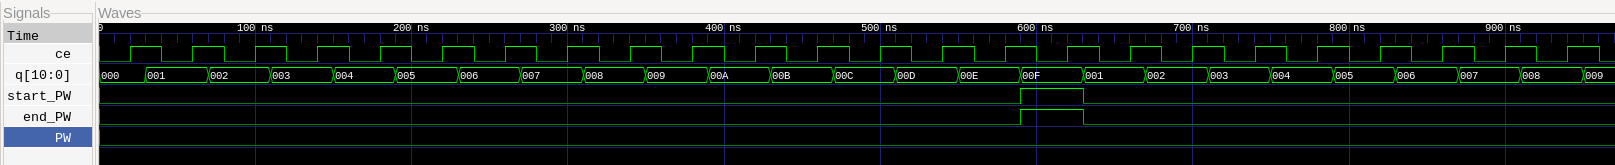
\includegraphics[scale=0.3]{../images/AGNMT_N=MT.png}
\end{center}

\begin{center}
	\textit{Рис. 2. Случай N<MT.}
	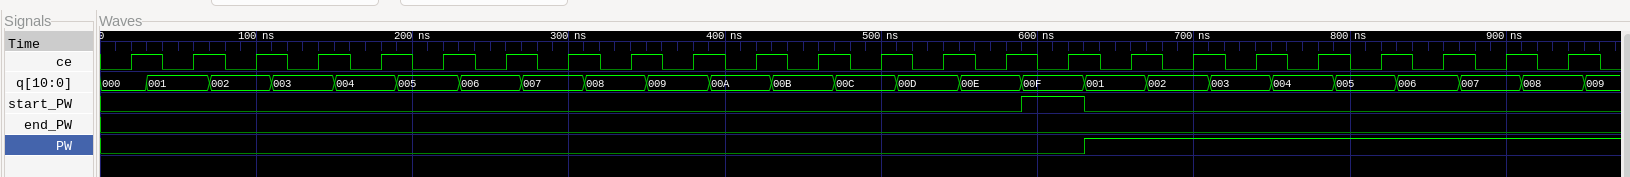
\includegraphics[scale=0.3]{../images/AGNMT_N<MT.png}
\end{center}

\textbf{\textit{\underline{2.3.}}} Начертить в тетради временные диаграммы генератора “пилы” AGSAW при Х=Y, X<Y.
\begin{center}
	\textit{Рис. 3. Случай X=Y.}
	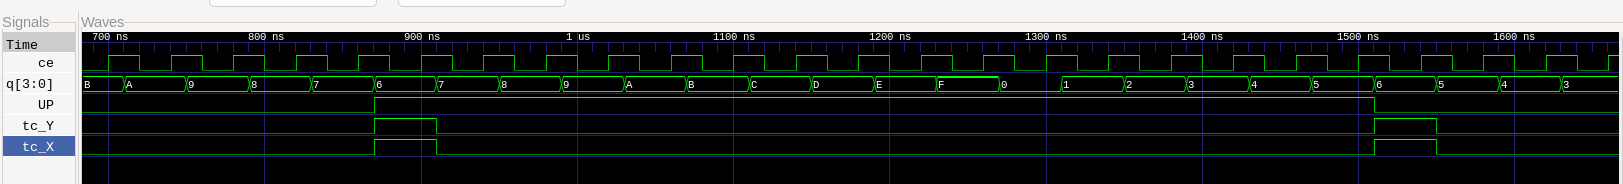
\includegraphics[scale=0.3]{../images/AGSAW_YX_X=Y.png}
\end{center}
\begin{center}
	\textit{Рис. 4. Случай X<Y.}
	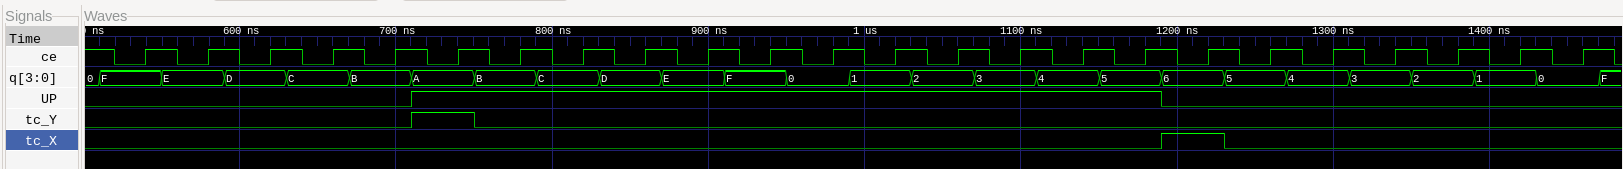
\includegraphics[scale=0.3]{../images/AGSAW_YX_X<Y.png}
\end{center}

\textbf{\textit{\underline{2.4}}} Начертить в тетради пример временных диаграмм аккумулятора Sch\_Lab402d, определить значение(я) периода аккумулятора при М=500 для своего Х согласно таблице.
\begin{center}
	\begin{tabular}{|c|p{2.5cm}|p{2cm}|p{2.5cm}|c|c|c|p{4cm}|}
		\hline
		№	& $NT_{clk}$ \scriptsize{(Период ce $T_{ce}=NT_{clk}*T_{clk}$)} & N\scriptsize{(Период $T_{per}=N*T_{ce}$)} & MT\scriptsize{(Длительность $T_{pw}=MT*T_{ce}$)}   & Y & X & {$\Delta F_{M_{x}}	$} [Hz] & Вариант измерения \\
		\hline
		4 & 5000 & 60 & 15 & 4 & 14 & 10 & PW/$T_{ce}$ (AGNMT) \\
		\hline
	\end{tabular}
\end{center}

\begin{center}
	\textit{Рис. 5. Временная диаграмма аккамулятора Sch\_Lab402d с табличными данными(JC3 - PW, ceo - $T_{ce}$)}
	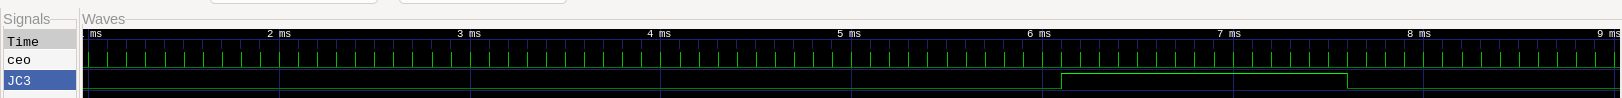
\includegraphics[scale=0.3]{../images/Sch_Lab402d.png}
\end{center}

Нетрудно заметить, что в таком случае искомая величина для символа AGNMT $PW/T_{ce}$ = 15. \\
Период аккамулятора определим в соответствии с формулой $M=\frac{F_{clk}}{2 \cdot \Delta F_{M_{x}} \cdot N_{T_{clk}}}$.\\
Отсюда получаем формулу $F_{clk}=2M\cdot\Delta F_{M_{x}} \cdot N_{T_{clk}}$. Подставим известные значения и получим $F_{clk} = 50$ MHz.\\

\title{\large{\textit{3. Задание к выполнению работы.}}}\\\\

\textbf{\textit{\underline{3.1.}}} Создать модуль ждущего генератора импульса WGMNT. Выполнить синтез, провести моделирование работы генератора. Зарисовать эскизы временных диаграмм.
\begin{center}
	\textit{Рис. 6. Временная диаграмма модуля WGNMT.}
	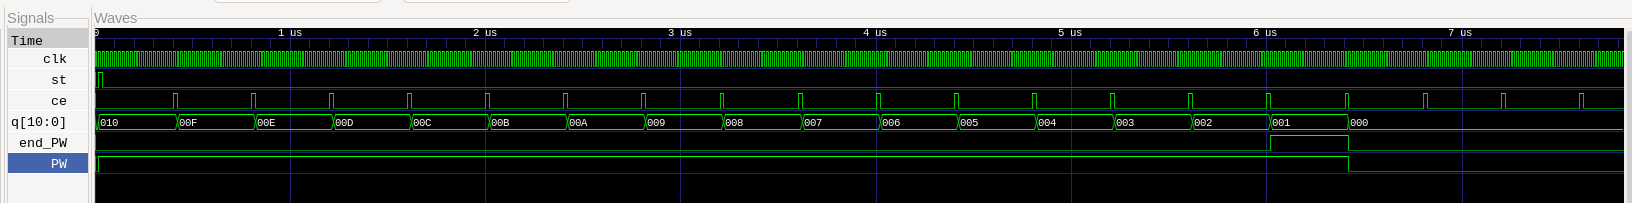
\includegraphics[scale=0.3]{../images/WGMT.png}
\end{center}

\textbf{\textit{\underline{3.2.}}}  Создать модуль AGNT выбранного варианта синтезатора периода. Выполнить синтез, провести моделирование работы генератора. Зарисовать эскизы временных диаграмм.
\begin{center}
	\textit{Рис. 7. Временная диаграмма модуля AGNT.}
	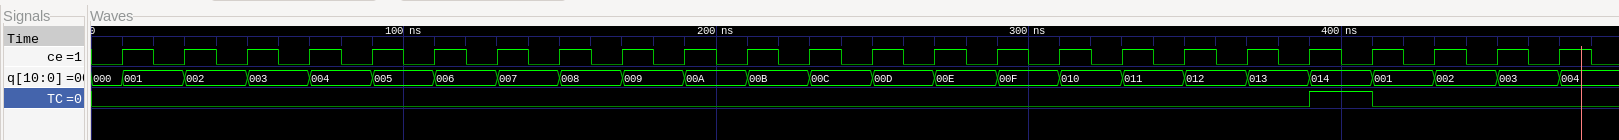
\includegraphics[scale=0.3]{../images/AGNT.png}
\end{center}

\textbf{\textit{\underline{3.3.}}} Создать модуль AGNMT генератора периодической последовательности импульсов с длительностью $MT \cdot T_{ce}$ и периодом $N \cdot T_{ce}$. Выполнить синтез, провести моделирование работы генератора. Зарисовать эскизы временных диаграмм.
\begin{center}
	\textit{Рис. 8. Временная диаграмма модуля AGNMT в случае N>MT.}
	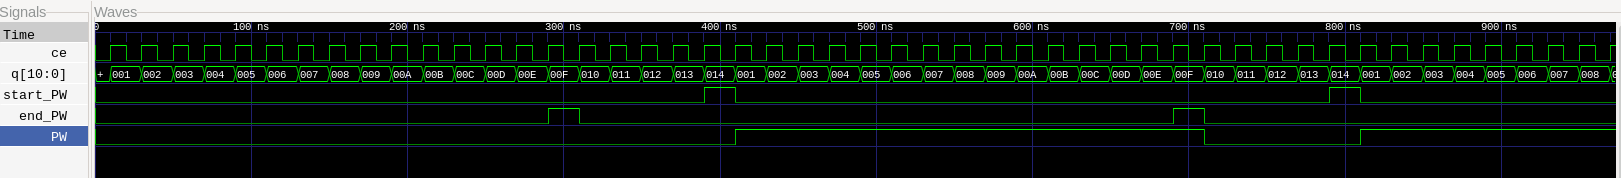
\includegraphics[scale=0.3]{../images/AGNMT_N>MT.png}
\end{center}

\textbf{\textit{\underline{3.4.}}} Создать модуль AGSAW генератора “пилы от Y до X ”. Выполнить синтез, провести моделирование работы генератора «пилы». Зарисовать эскизы временных диаграмм.
\begin{center}
	\textit{Рис. 9. Временная диаграмма модуля AGSAW в случае X>Y.}
	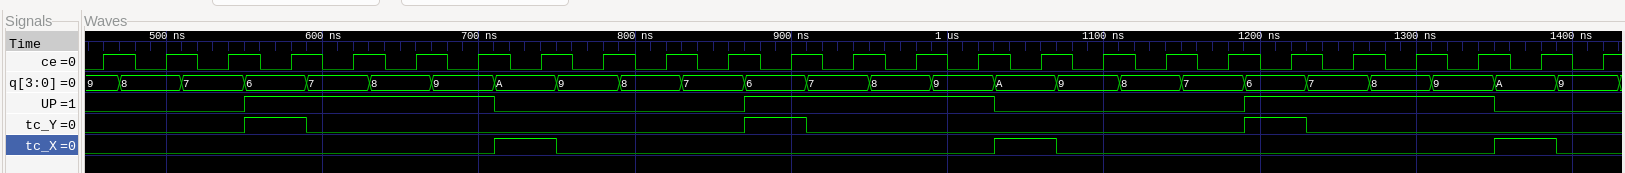
\includegraphics[scale=0.3]{../images/AGSAW_YX_X>Y.png}
\end{center}

\textbf{\textit{\underline{3.5.}}} Создать модуль ACC2mE аккумулятора с емкостью $2^{m}$. Выполнить синтез, провести моделирование работы генератора. Зарисовать эскизы временных диаграмм.
\begin{center}
	\textit{Рис. 10. Временная диаграмма модуля ACC2mE.}
	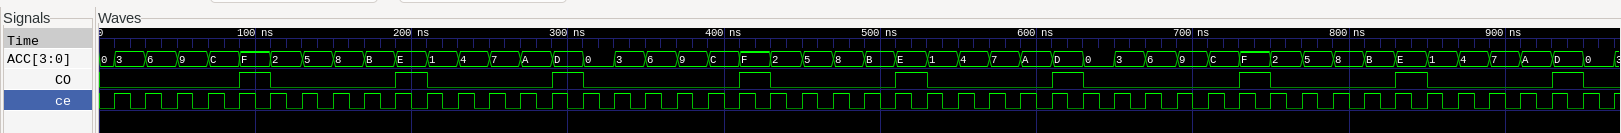
\includegraphics[scale=0.3]{../images/ACC2mE.png}
\end{center}

\textbf{\textit{\underline{3.6.}}} Для заданных параметров создать символы всех отлаженных модулей. \\

\textbf{\textit{\underline{3.6.1}}} Создать модуль ACCM (1.5.2). Для заданных $\Delta F_{M_{x}}$ и $NT_{clk}$ определить M. Создать символ этого модуля. M = 500.
\begin{center}
	\textit{Рис. 11. Временная диаграмма модуля ACCM.}
	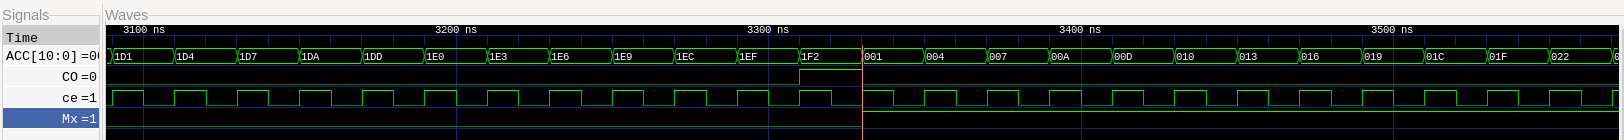
\includegraphics[scale=0.3]{../images/ACCM.png}
\end{center}

\textbf{\textit{\underline{3.7.}}} Для заданных параметров создать модуль и символ DAT\_BL. \\

\textbf{\textit{\underline{3.8.}}} Создать модуль и символ BUTTON\_BL. \\

\textbf{\textit{\underline{3.9.}}} Создать модуль и символ Display. \\

\textbf{\textit{\underline{3.10.}}} Из созданных символов составить схему Sch\_Lab402d. Без модуля MEG\_BL на вход HB[7:0] старшего байта семи сегментного индикатора Display можно подать 8 бит шины N[7:0] или MT[7:0]. Выполнить синтез схемы Sch\_Lab402. \\

\textbf{\textit{\underline{3.11.}}} Проверить работу всех генераторов импульсов. Получить и сохранить осциллограммы выходных сигналов:
\begin{itemize}
	\item PW и end\_PW - ждущего генератора WGMT;
	\item TC – синтезатора периода AGNT или AGNTD;
	\item PW – генератора AGNMT;
	\item Udac – макета ЦАП DAC\_R2R;
	\item CO и Mx – синтезатора частоты ACCM.
\end{itemize}
\begin{center}
	\textit{Рис. 12. Данные симуляции для модуля Sch\_Lab402d(WGMT:PW/end\_Pw=JA1/JA3, AGNT: TC=JA4, AGNMT: PW=JC3, ACCM: CO/$M_{x}$=JD3/JD4).}
	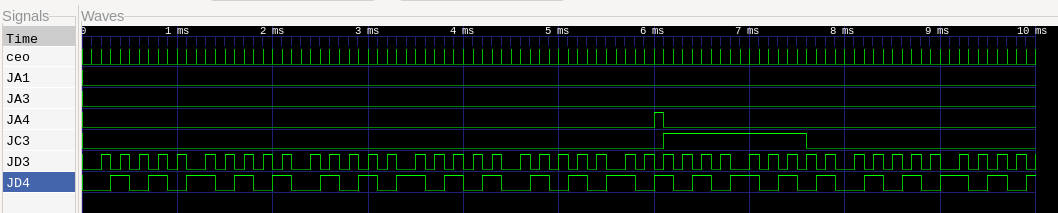
\includegraphics[scale=0.5]{../images/Sch_Lab402d_data.png}
\end{center}

\title{\large{\textit{4. Задания к сдаче работы.}}}\\\\

\textbf{\textit{\underline{4.1.}}} Составить схему модуля MEG\_BL измерителя параметров импульсов заданного варианта генератора. Модуль MEG\_BL должен иметь 5 портов входов: clk, st, Inp, REF, res и один 8-и битный выходной порт Q[7:0]. Вход res должен обеспечивать «сброс»
результатов измерений. Измерители частоты сигналов аккумулятора и генератора меандра не должны иметь погрешность дискретности отсчета. \\
Выход Q[7:0] результатов измерения модуля MEG\_BL предназначен для соединения с входом старшего байта HB[7:0] модуля Display. \\
Запускаться измеритель должен по входу st сигналом с выхода модуля BUTTON\_BL. \\
На вход Inp должен подаваться измеряемый сигнал, а на вход REF эталон времени:
\begin{itemize}
	\item се – при измерениях длительности или периода;
	\item PW – при измерении частоты.
\end{itemize}

\textbf{\textit{\underline{4.2.}}} Создать модуль MEG\_BL провести моделирование его работы. Зарисовать эскиз полученных временных диаграмм.
\begin{center}
	\textit{Рис. 13. Временная диаграмма модуля MEG\_BL.}
	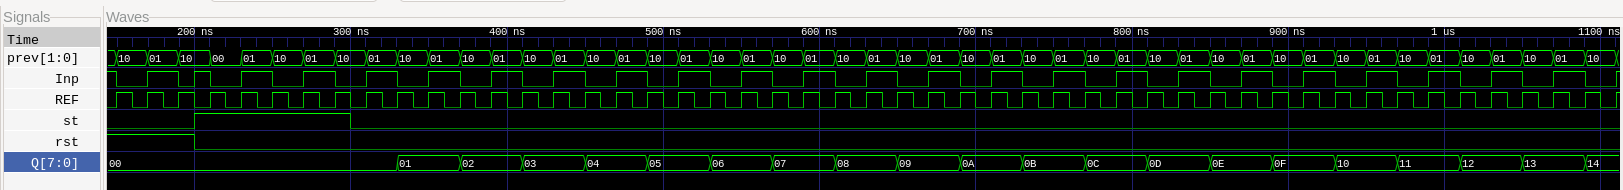
\includegraphics[scale=0.3]{../images/MEG_BL.png}
\end{center}

\textbf{\textit{\underline{4.3.}}} Создать символ MEG\_BL, вставить его в лист схемы Sch\_Lab402. Создать файл конфигурации (Generate Target PROM/ACE File) загрузить в ПЛИС или ПЗУ макета. Продемонстрировать работу измерителя.

\textbf{\textit{\underline{4.2.}}} Создать модуль MEG\_BL провести моделирование его работы. Зарисовать эскиз полученных временных диаграмм.
\begin{center}
	\textit{Рис. 14. Результат симуляции итогового модуля Sch\_Lab402.}
	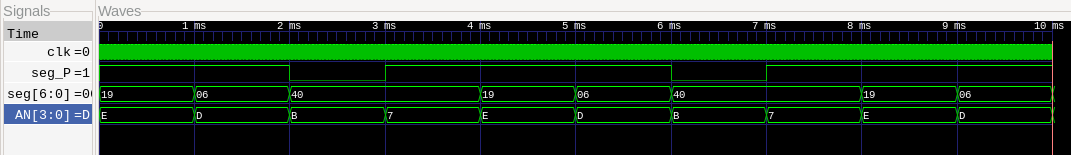
\includegraphics[scale=0.45]{../images/result.png}
\end{center}

\end{document}
